\documentclass[UTF8]{ctexart}
\usepackage[vmargin=2.5cm]{geometry}
%\usepackage{abstract} %生成摘要使用的宏包
\usepackage[colorlinks,linkcolor=black,anchorcolor=black,citecolor=black]{hyperref} %“colorlinks”的意思是将超链接以颜色来标识,而并非使用默认的方框来标识。linkcolor,anchorcolor, citecolor分别表示用来标识link, anchor, cite等各种链接的颜色。此处我们均设为黑色。
\usepackage{fancyhdr} %插入页脚的宏包
\usepackage{graphicx}%图片宏包
\usepackage{float}
\usepackage{subfigure}%并列插入图片
\usepackage{amsmath}%公式宏包
\usepackage[T1]{fontenc}% 统一修改正文和数学字体为Adobe Utopia, 这个字体和Times有些像
\usepackage{newtxtext, newtxmath}  %两种使用Times New Roman 字体的方法
\usepackage{appendix}%加入附录需使用appendix宏包
\usepackage{listings}%插入代码
\usepackage{color}

\graphicspath{{./Figs/}}
\DeclareGraphicsExtensions{.pdf,.jpeg,.png,.jpg}%在添加图片后只需要图片的名字,而不需要拓展名
\linespread{1.5}%设置行间距为1.5倍行距

\renewcommand{\abstractname}{\Large\textbf{摘要}}

%---------文档的开始,一定要有文档的结束,才能生效-----------
\begin{document}

%-------------------------标题-------------------------
\begin{titlepage}%使页码跳过这页
\begin{center}
\heiti\zihao{3}\textbf{基于最小二乘回归模型的红外光谱溶液浓度预测} %标题3号加粗
\vspace{2ex}
\end{center}

%-------------------------摘要部分-------------------------
\begin{abstract}
最小二乘回归模型通过最小化误差的平方和寻找数据的最佳函数匹配,可以简便地求得未知的数据,并使得这些求得的数据与实际数据之间误差的平方和为最小,因此本文选用最小二乘回归模型作为矫正模型。我们将$\frac{2}{3}$ 的数据用于训练集合,剩下$\frac{1}{2}$的数据用于检测集合。我们发现吸光度-波长图像下方的数据预测效果良好,上方的数据预测效果。\par
最后,我们对本模型进行评价,提出了可以用偏最小二乘、机器学习算法进行预测的展望。\par
\textbf{关键词:}红外光谱;Savitzky-Golay平滑处理;混合溶液浓度检测;预测模型;普通最小二乘回归模型
\end{abstract}
\end{titlepage}

%-------------------------正文部分-------------------------
%修改页眉页脚
\pagestyle{fancy}
\lhead{}
\chead{}
\rhead{}
%\lfoot{}
\cfoot{第\thepage 页}
%\rfoot{} %空格即表示空白
\renewcommand{\headrulewidth}{0pt}
\renewcommand{\footrulewidth}{0.4pt} %设置页眉页脚分割线的宽度,如果为0pt,则不显示线条

%-------------------------问题重述-------------------------
\newpage
\section{问题重述}
目前有两种溶液U(VI)和U(VI)按照一定的浓度与硝酸溶液混合。经过红外光线扫描,得到该混合溶液在一定波长下的频谱。试根据现有频谱数据建立预测两种溶液的浓度的数学模型,并用该模型预测出待检混合溶液样本中的两种溶液的浓度。\par

%\subsection{1.xx}
%\subsubsection{1.1xx}
%-------------------------问题分析-------------------------
\section{问题分析}
\subsection{光谱数据预处理}
\subsubsection{数据的平滑处理}
\subsubsection{聚类分析}
混合溶液的光谱图呈现明显的上下分离趋势,因此我们使用K-means聚类算法将频谱数据分成2类,分别建立模型,寻找参数,提高预测效果。

\subsection{预测模型建立与检验}
普通最小二乘法通过最小化误差的平方和寻找数据的最佳函数匹配,可以简便地求得未知的数据,并使得这些求得的数据与实际数据之间误差的平方和为最小,较为常用。在本题中,我们选择普通最小二乘法模型作为预测模型。我们仅利用$ \frac{2}{3} $的数据集来建立模型,剩下$ \frac{1}{3} $的数据集用来对模型进行误差检验,识别模型预测效果。

\subsection{预测待检混合溶液浓度}
模型建立与误差检验完成后,使用该模型预测出待检混合溶液样本中的两种溶液的浓度。研究思路如\ref{fig:1}所示。

\begin{figure}[htbp]
	\centering
	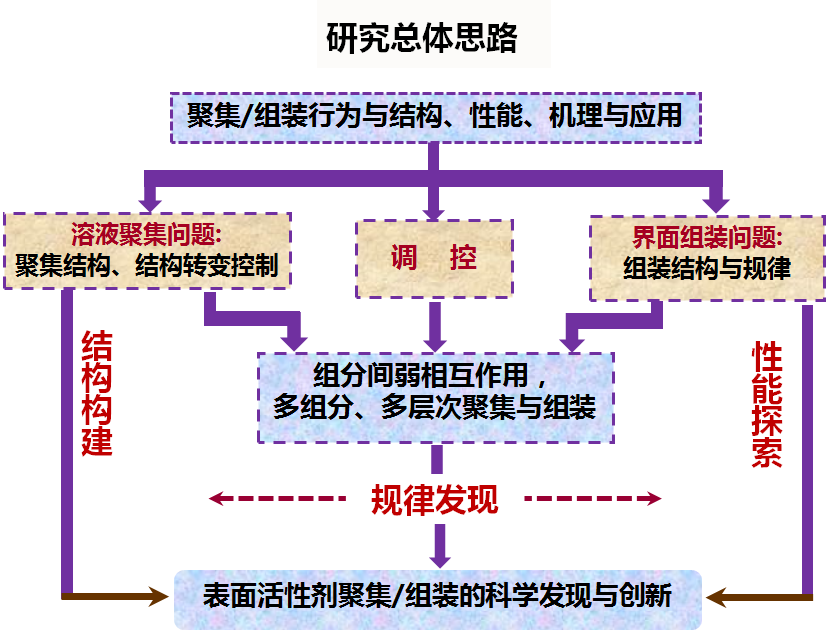
\includegraphics[width=1.0\linewidth]{flow.png}
	\caption{研究思路图}
	\label{fig:1}
\end{figure}

%-------------------------模型假设-------------------------
\section{模型假设}

%带标号的列表
\begin{enumerate}
	\item 扫描溶液的红外光线是平行单色光。
	\item 本文涉及的溶液均为均匀的、非散射的吸光物质溶液。
	\item 每次测量的光程不变。
\end{enumerate}

%-------------------------符号说明-------------------------
\section{符号说明}

%本部分是对模型中使用的重要变量进行说明,一般排版时要放到一张表格中。
%注意:第一:不需要把所有变量都放到这个表里面,模型中用到的临时变量可以不放。第二:下文中首次出现这些变量时也要进行解释,不然会降低文章的可读性。
%使用三线表格最好~
\begin{table}[H]
\centering
\caption{这是一个表格}
    \begin{tabular}{p{4.5cm} p{4.5cm} p{4.5cm}}%htbp表示的意思是latex会尽量满足排在前面的浮动格式,就是h-t-b-p这个顺序,让排版的效果尽量好。
		%指定单元格宽度, 并且水平居中。
		\hline
		符号 & 说明 & 单位 \\ %换行 
		\hline
		$\int$ & 积分符号 &  \\ %把你的符号写在这
		$W_0$ & 区分高峰和低峰的一个临界值 &  \\ %把你的符号写在这
		$M_t$ &  简单移动平均项 &  \\ %把你的符号写在这
		\hline
	\end{tabular}
\end{table}

%---------------------模型的建立与求解---------------------
\section{模型的建立与求解}
\subsection{红外光谱检测方法}

含有各类官能团和化学键的化学物质对各类光的吸收、散射、发射的特征不同,因此可以用来了解其组成特点和数量\cite{02}。由于技术和应用的不同,通常把红外光谱区划分为3个区:近红外区,中红外区和远红外区。近红外光谱区位于 $ 780 \sim  2500 nm $,是人们认识最早的非可见光光谱,其中位于$ 780 \sim 1100nm $的光谱区域称为短波近红外区,位于$ 1100 \sim 2526nm $的光谱区域称为长波近红外区,如\ref{fig:22}所示。近红外光谱技术具有测量过程简单、分析速度快、成本低、效率高、样品不需要预处理、可同时测定样品的多个组分、测量重现性好等特点。

\begin{figure}[htbp]
	\centering
	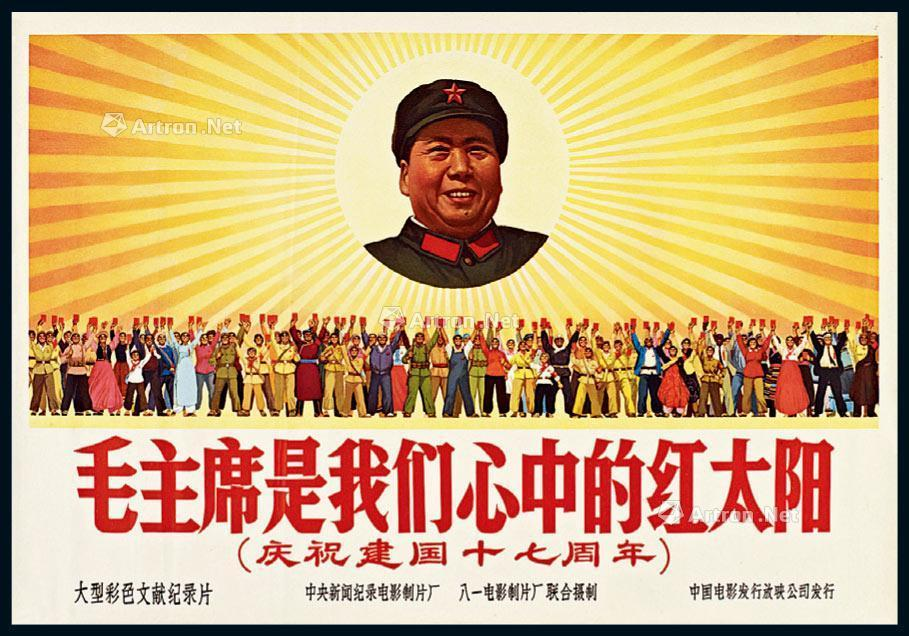
\includegraphics[width=1.0\linewidth]{sunlights.jpg}
	\caption{近红外光谱区在电磁波中的位置}
	\label{fig:22}
\end{figure}

分子的非谐振性振动使得分子振动从基态向高能级跃迁,近红外光谱由此产生,主要记录含氢基团 (C-H、O-H、N-H、S-H、P-H等) 振动的倍频和合频吸收。近红外光通过待测样品时,不同样品具有不同的基团组成及含量,对应的近红外光的吸收程度也不同。光吸收的程度通常用吸光度 A (Absorbance)来表示,指光线通过某一溶液或物质前的入射光强度与该光线通过溶液或物质后的透射光强度比值的对数。朗伯-比尔定律 (Beer-Lambert Law) 可以定量描述样本吸光度特性,是近红外光谱分析技术的基础,其表达式为:\par

\begin{equation}
	 A= log\left( \frac{I_{0} }{I_T}\right ) =log\left( {\frac{1}{T} } \right )= Kbc,
\end{equation}
其中:\\
$ A $: 吸光度;\\
$ I_{t} $: 入射光强度;\\
$ T $: 为透射比 (透过光强度比入射光强度);\\
$ c $: 被测样品组分浓度;\\
$ b $: 液层厚度;\\
$ K $: 比例常数,与入射光的波长,待测物质的性质和溶液的温度等因素有关。 \\

当一束平行单色光垂直通过某一均匀、非散射的吸光物质溶液时,其吸光度 $ A $ 与溶液液层厚度 $ b $ 和样品浓度 $ c $ 的乘积成正比。\par

\subsection{数据预处理}
\subsubsection{数据除噪}
本题提供了两种溶液用红外光线扫描后在一定波长下的频谱数据和待测溶液样本的光谱数据。对光谱的三次测量进行平均后得到的结果如 图 \ref{fig:3} 所示。通过观察图像, 我们发现数据在峰值位置存在明显的振荡,故需要对数据进行平滑处理。

平滑处理可以使数据变得更加平滑,便于进一步的分析和理解,有效减少数据中的噪声和异常值,提高数据的可靠性和准确性。我们分别采用Movmedian平滑处理、五点三次平滑处理、Savitzky-Golay (SG)平滑处理,然后对此三种处理的结果进行比较,选择处理效果最好的方法。

\{Insert Figure 3 here.\}

\subsubsection{分类分析}
由于聚类分析后的结果与图像不符,我们以光谱数据$ 900nm $处的浓度作为分类标准,浓度大于1的为一类,浓度小于1的为一类,分类后的效果如图9所示。\par


%-------------------------模型分析-------------------------
\section{模型分析}
%并列放置多张图片
\begin{figure}[H]
	\centering
	\subfigure[]%加入[]即可给小图片自动编号
	{
		\begin{minipage}[b]{.3\linewidth}%第一张图片占宽的1/3
			\centering
			\includegraphics[width=1.0\linewidth]{yby01.jpg}
		\end{minipage}
	}
	\subfigure[]
	{
		\begin{minipage}[b]{.3\linewidth}
			\centering
			\includegraphics[width=1.0\linewidth]{yby02.jpg}
		\end{minipage}
	}
	\subfigure[]
	{
		\begin{minipage}[b]{.3\linewidth}
			\centering
			\includegraphics[width=1.0\linewidth]{yby03.jpg}
		\end{minipage}
	}
	\caption{并列放置的3张江苏园博园图@20231029}
	\label{fig:3}
\end{figure}

%-------------------------模型总结-------------------------
\section{模型总结}
\subsection{模型的优点}
\subsection{ 模型的缺点}
\subsection{模型的推广与改进}
这篇文章结束了!

\newpage
%-------------------------参考文献-------------------------
%\bibliographystyle{plain} %参考文献的排版格式
%\bibliographystyle{reference} 
%参考文献的位置
\begin{thebibliography}{9} %{99}表示添加参考文献数量的宽度,任意两位数字的参考文献就可以输入99
	\bibitem{01}熊婵. 基于多维多模式超光谱系统的复杂混合溶液成分分析[D]. 天津大学, 2012.
    \bibitem{02}谈爱玲. 水中石油类污染物光纤光谱检测方法的研究[D]. 燕山大学, 2012.
	\bibitem{03}孙明顺. 毕赤酵母发酵过程中甲醇浓度的红外光谱分析方法研究[D]. 山东大学, 2016.
%	\bibitem{04}
%	\bibitem{05}
%	\bibitem{06}
\end{thebibliography}
%正文中引用到参考文献的地方\cite{01} \cite{02}

%-------------------------附录部分-------------------------
% 使用\begin{appendices} \end{appendices} 或者直接用\appendix
\appendix
%代码格式设置,代码的设置与具体的编程语言有关,比赛时上网搜素即可
\definecolor{dkgreen}{rgb}{0,0.6,0}
\definecolor{gray}{rgb}{0.5,0.5,0.5}
\definecolor{mauve}{rgb}{0.58,0,0.82}
\lstset{ %
	language=Python,                % the language of the code
	basicstyle=\footnotesize,           % the size of the fonts that are used for the code
	numbers=left,                   % where to put the line-numbers
	numberstyle=\tiny\color{gray},  % the style that is used for the line-numbers
	stepnumber=2,                   % the step between two line-numbers. If it's 1, each line 
	% will be numbered
	numbersep=5pt,                  % how far the line-numbers are from the code
	backgroundcolor=\color{white},      % choose the background color. You must add \usepackage{color}
	showspaces=false,               % show spaces adding particular underscores
	showstringspaces=false,         % underline spaces within strings
	showtabs=false,                 % show tabs within strings adding particular underscores
	frame=single,                   % adds a frame around the code
	rulecolor=\color{black},        % if not set, the frame-color may be changed on line-breaks within not-black text (e.g. commens (green here))
	tabsize=2,                      % sets default tabsize to 2 spaces
	captionpos=b,                   % sets the caption-position to bottom
	breaklines=true,                % sets automatic line breaking
	breakatwhitespace=false,        % sets if automatic breaks should only happen at whitespace
	title=\lstname,                   % show the filename of files included with \lstinputlisting;
	% also try caption instead of title
	keywordstyle=\color{blue},          % keyword style
	commentstyle=\color{dkgreen},       % comment style
	stringstyle=\color{mauve},         % string literal style
	escapeinside={\%*}{*)},            % if you want to add LaTeX within your code
	morekeywords={*,...}               % if you want to add more keywords to the set
}
\section{附录}
\subsection{问题一}
\begin{lstlisting}
q=2;w=2;e=2;
X(:,1)=X(:,1).^q;
X(:,2)=X(:,2).^w;
X(:,3)=X(:,3).^e;
Y=nongdu_up(1:56,:);
[B]=OLS(Y,X)
x=unknownabs';
for j=1:7
X1(:,j)=x(:,upi(j,2));
end
Y0=X1*B;
\end{lstlisting}
\subsection{问题二}
\subsection{问题三}
\subsection{问题四}
\subsection{参数可靠性检验}

%-------------------------补充部分-------------------------
\newpage
1. 插入表格
\begin{center}
	\textbf{表1 描述性统计}
	
	\vspace{3pt}
	\begin{tabular}{clllll} %c居中 l左对齐 r右对齐
		\hline %两个\hline表示双横线
		a &c1 &c2 &c3 &c4 &c5\\
		\hline
		a &c1 &c2 &c3 &c4 &c5\\
		a &c1 &c2 &c3 &c4 &c5\\
		a &c1 &c2 &c3 &c4 &c5\\
		a &c1 &c2 &c3 &c4 &c5\\
		a &c1 &c2 &c3 &c4 &c5\\
		a &c1 &c2 &c3 &c4 &c5\\
		a &c1 &c2 &c3 &c4 &c5\\
		\hline		
	\end{tabular}
\end{center}

2. 公式对齐

$$
\left\{
\begin{aligned}
y&=1, & -1<x&<4, \\
y&=2, &    x&>6, \\
y&=3, & -5<x&, 
\end{aligned}
\right.
$$
\end{document}